\newpage

\setcounter{page}{1}
\makecvfooter
  {Jerald Thomas}
  {Research Statement}
  {Page \thepage \hspace{1pt} of \pageref{research_last}}


\makecvheader[C]
%\doublespacing

\cvsection{Research Statement}

In 1965, Ivan Sutherland published his seminal paper, ``The Ultimate Display", which set a community-wide vision of what the future of virtual and augmented reality holds. Since then, researchers have seen the potential for immersive technologies to transform how people work, communicate, and entertain themselves. These potentials are beginning to be realized thanks to modern technology; this is evident by the significant impact virtual reality and other immersive technology devices have made on the consumer electronics market in the last decade. However, several practical and theoretical problems still need to be solved to meet the public’s expectations, resulting in immersive technologies restricted by how and where people can use them. The overarching goal of my research is to address fundamental usability problems of virtual and augmented reality, allowing for technologies that are more generalizable and applicable to the user's current situation and environment. My work specifically focuses on developing and evaluating user interface techniques that make use of the user's physical surroundings rather than avoiding them, and in doing so, making these technologies more compelling and accessible to a larger population. This is done by creating and using forward-thinking human-computer interaction techniques and evaluating them with thorough and well-designed empirical studies. Broadly, my current research agenda can be divided into two themes: locomotion and collaboration. Other research interests of mine that I am excited to incorporate into my research agenda in the future include human-robot interaction, immersive technology assisted therapy, and computer science education.

\section*{Locomotion and Redirected Walking}
\vspace{-0.25cm}

In my locomotion research, I focus on a virtual reality based technique called redirected walking. Redirected walking augments a technique known as natural locomotion, in which a user's physical movements (translation and rotation) are directly applied to their virtual perspective, thus allowing them to explore their virtual environment in a way that is more typical to their real-world experiences when compared to other locomotion methods. Redirected walking works by introducing small discrepancies between the user's perceived motions (their virtual path) and their actual motions (their physical path). When leveraged correctly, these discrepancies can make greater use of the user's physical environment.

My dissertation, which was nominated for the 2023 IEEE VGTC Virtual Reality Best Dissertation Award, focused entirely on redirected walking and provided several contributions. Of these, there are three primary contributions that I consider to be most important. I first introduced a new class of algorithms that allow redirected walking to work in physical environments that have obstacles or non-convex boundaries, which was not possible in a generalizable manner before \cite{thomas2019general}. This work uses techniques from the robotics literature, most notably artificial potential fields. The technique that I introduced has been derived and improved upon by the redirected walking community and has become the defacto standard for redirected walking algorithms. Next, I sought to not just allow for physical obstacles when using redirected walking, but to actually incorporate them into the redirected walking experience \cite{thomas2020towards, thomas2020reactive, thomas2022inverse}. The most common example would be for passive haptic feedback, in which a user interacts with a virtual object that has a tracked physical object ``tied'' to it, giving the interaction an incredible sense of realism. However, because redirected walking does not maintain a 1:1 mapping between the user's physical and virtual movements, these types of interactions are not generally possible. My dissertation introduces the concept of ``alignment'', which uses redirected walking techniques to not only keep users away from obstacles and boundaries, but also to re-align the virtual and physical worlds so physical interactions are possible (Figure \ref{fig:alignment}). The paper introducing alignment won the best paper award at the 2020 ACM Symposium on Virtual Reality Systems and Technologies and has gone on to inspire several derivative works. Finally, my dissertation provides the first example of exploring usability considerations for creators designing redirected walking experiences \cite{thomas2022inverse}. The design of virtual reality experiences that incorporate redirected walking is non-trivial; this is a primary reason for industry's general lack of willingness to adopt redirected walking. Exploring and evaluating new means to assist with the creation of redirected walking experiences will be important for future redirected walking research, and my dissertation provides a solid foundation for doing so. My dissertation improves the current state of redirected walking by introducing novel redirected walking algorithms, and perhaps more importantly, new ways to use them.

\begin{figure}[!htb]
  \centering
  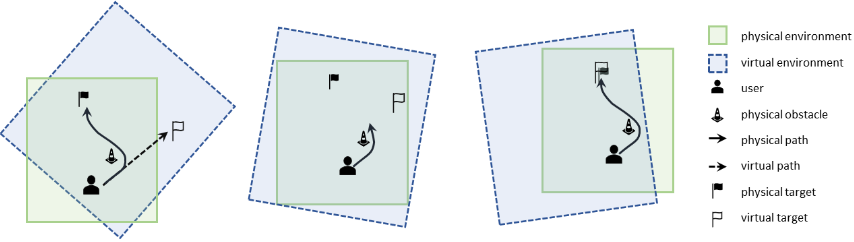
\includegraphics[width=.8\textwidth]{figures/alignment.png}
	\caption[]{A demonstration of environmental alignment with obstacle avoidance. 
	The left image shows the perceived path to a virtual target and the physical path to a proxy target.
	The middle and right images show the progression of the physical path to environmental alignment.
	When this occurs, the user can interact with the proxy target substituting for the virtual target.}
  \label{fig:alignment}
\end{figure}

Currently, my work regarding redirected walking is in two lines of research. First, I am collaborating with researchers at Miami University and the University of Maryland to deeply explore the use of simulation for evaluating redirected walking techniques. Using simulation for redirected walking evaluations is a fairly common practice, though there is little understanding of what exactly is lost when compared to live-user evaluations. We also do not fully understand what aspects of actual human locomotion have the greatest impact on redirected walking effectiveness. We are developing new methods to gain a better understanding of these problems. The first paper in this new line of research is nearing completion with a plan to submit to IEEE Transactions on Visualization and Computer Graphics (TVCG). I am also working with collaborators at Virginia Tech on developing new techniques for determining when a user notices the manipulation imparted by redirected walking. The most common practice when implementing redirected walking is that these manipulations should not be noticed by the user, but determining when a user notices them is a non-trivial task. Traditionally, a psychophysical technique is used where several users are presented with several levels of stimulus, and they self-report when they notice the manipulation. This technique has been shown to have a large degree of variability and does not provide results that persist as virtual reality hardware improves. Alternatively, the new technique I am developing uses eye tracking to determine when a user notices the manipulation by leveraging the user's vestibulo-ocular reflex. This will provide individual results that adapt with the user and their hardware. It will also give us greater insight into how and why users notice the manipulations in the first place. This work is fairly new and the user study is just beginning. Looking forward, these lines of research have the potential to produce several novel and important research contributions, and we are actively seeking grant funding for both of them.


\section*{Collaboration and Remote Physicality}
\vspace{-0.25cm}
As a postdoc, I now have the opportunity begin broadening my research scope to include topics other than redirected walking. The first direction I am excited to explore is the use of immersive technologies to facilitate collaboration. Particularly, I am interested in the concept of remote physicality, or how we incorporate the physical environment of all users to improve their collaboration experience. I am currently leading two projects that fall under this category. The first involves aligning the user's physical environments so that their combined shared environment is spatially coherent for all users. We are nearing the end of the exploration phase of this research, and we should be preparing to start a user study in the near future. I am also supervising a directed research project which seeks to create novel augmented reality user interfaces that maintain synchrony of pairs of remote physical objects. This would allow users in different physical environments to still use physical objects in their collaboration process. I recently led a team of researchers from Virginia Tech and Iowa State University in a grant proposal submitted to the NSF Research on Emerging Technologies for Teaching and Learning (RETTL) solicitation that will allow me to continue these projects and start others in this area of research. This grant proposal focuses on hybrid learning situations where some participants are remote and some are colocated in the context of Industrial Design pedagogy (Figure \ref{fig:rettl}).

\begin{figure}[!htb]
  \centering
  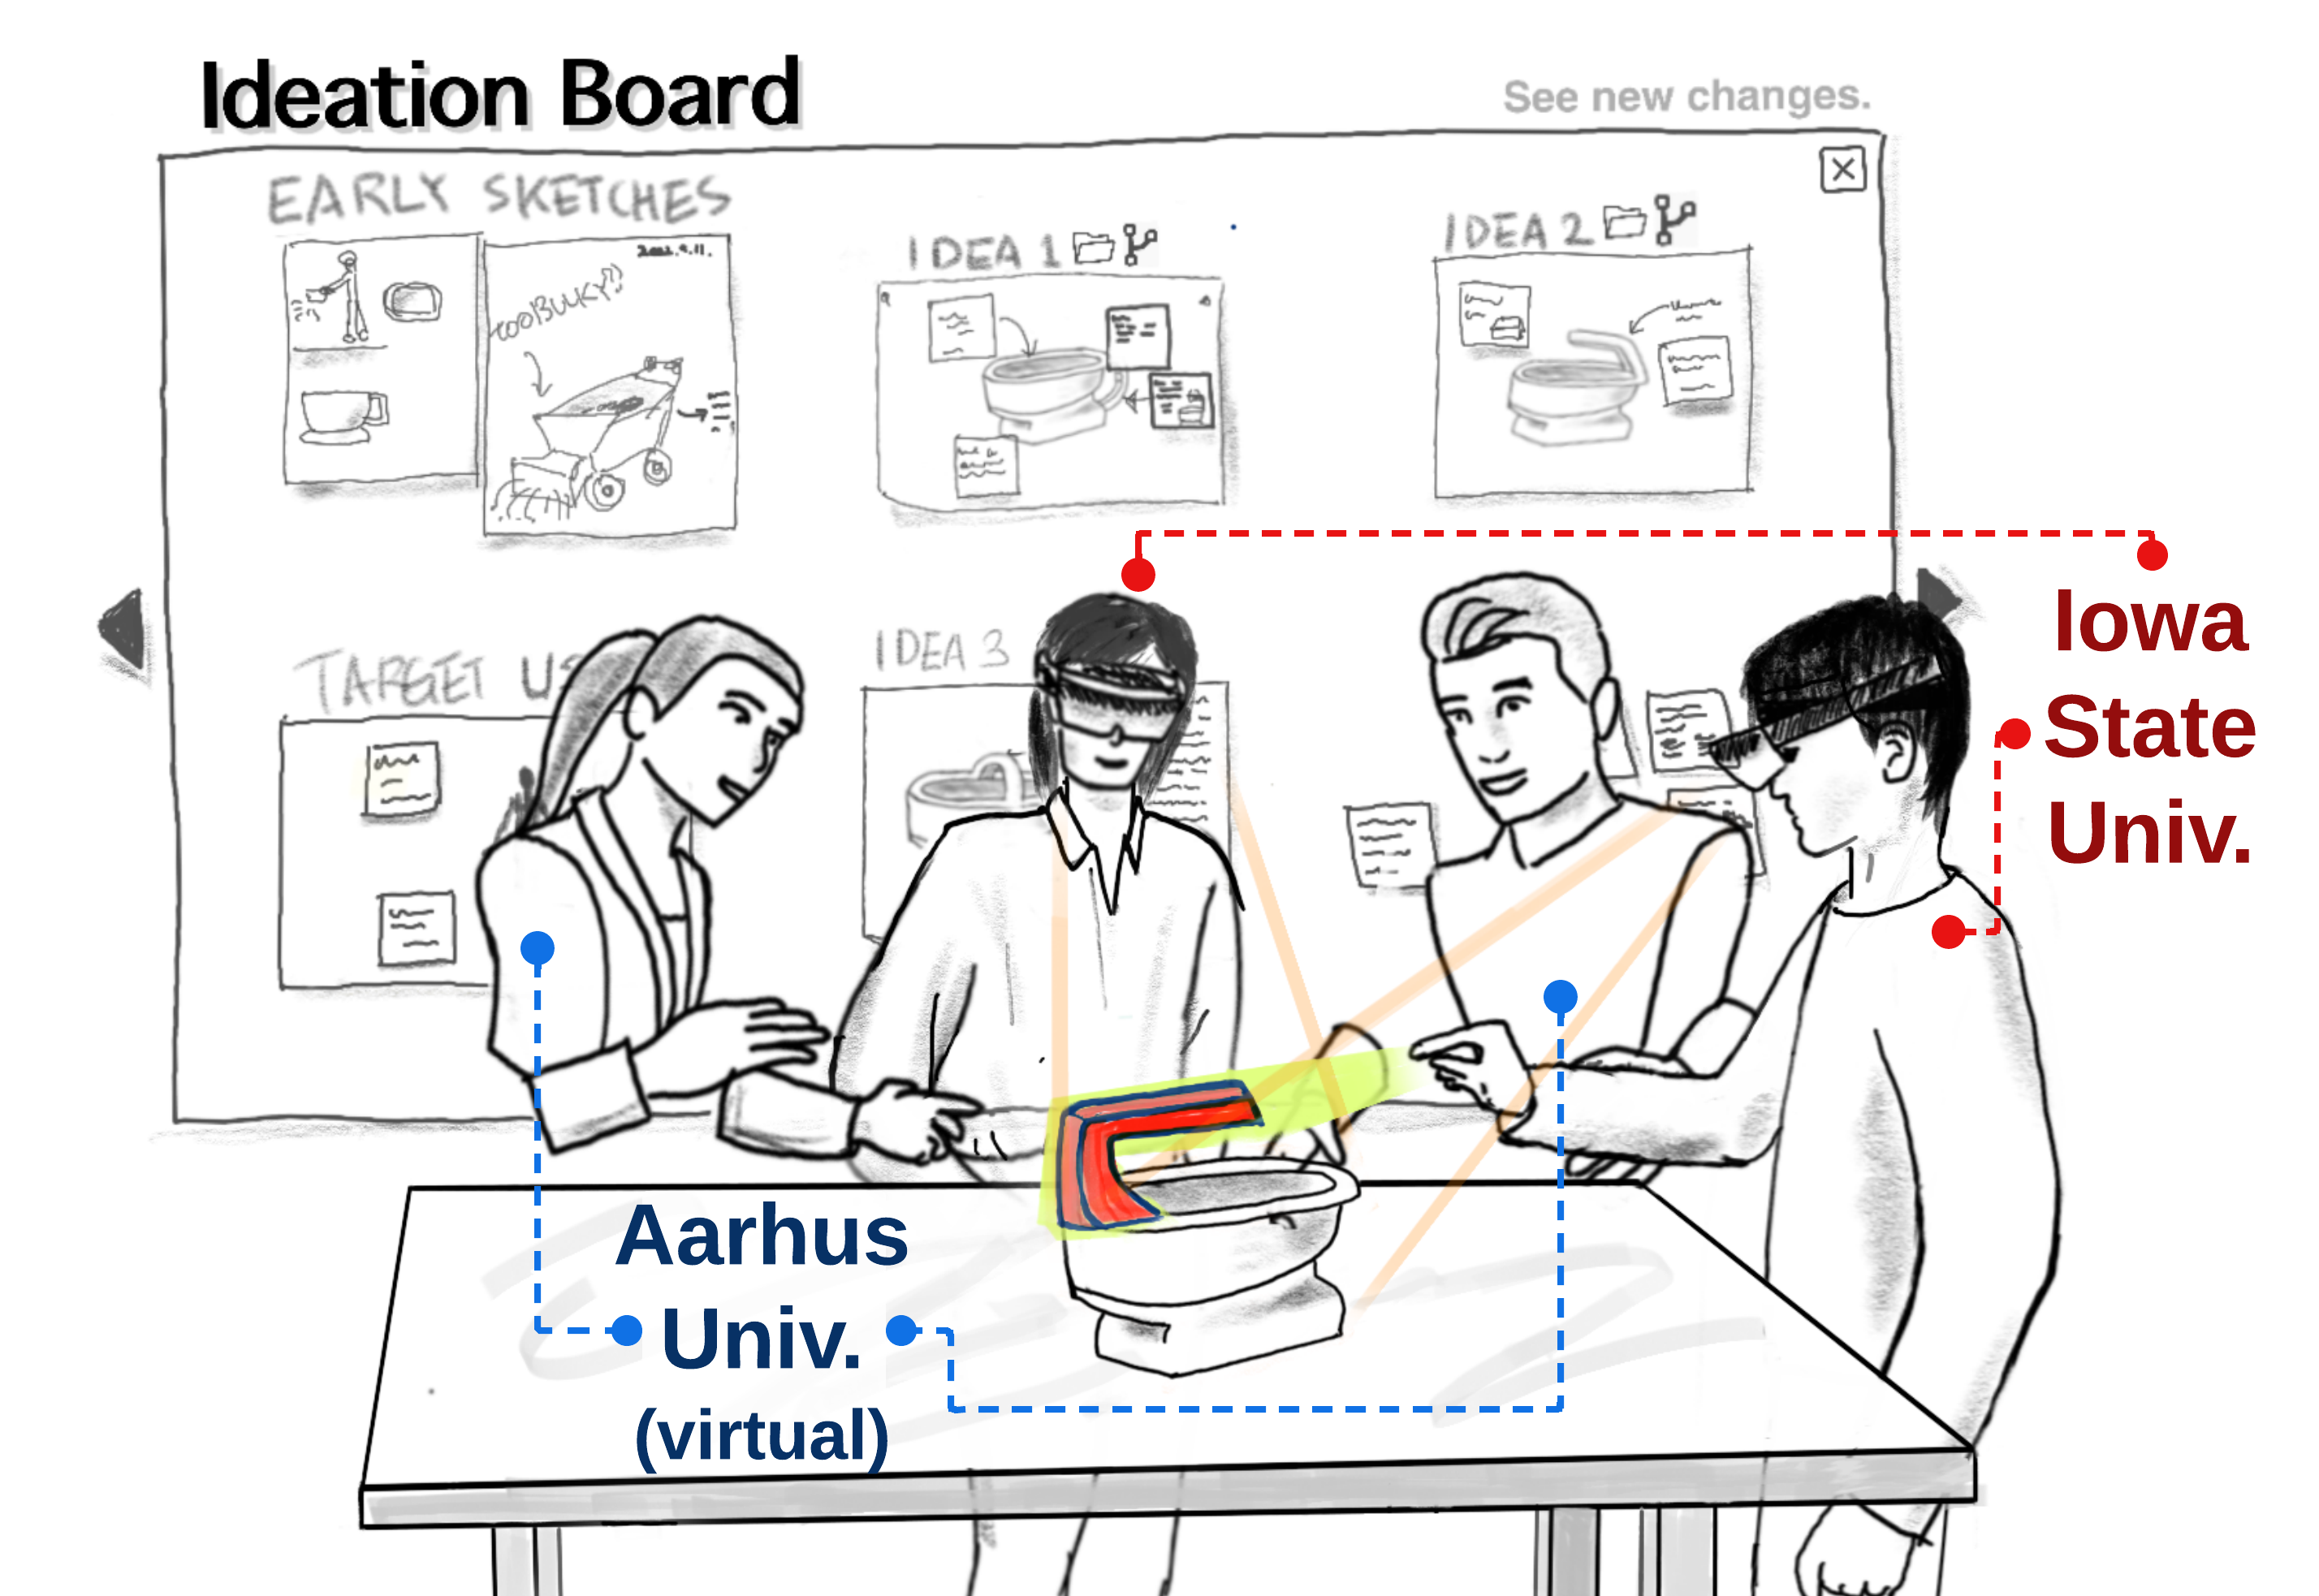
\includegraphics[width=.75\textwidth]{figures/rettl.png}
	\caption[]{An example use case highlighted in our NSF RETTL proposal of how immersive technologies can improve hybrid collaboration for industrial design education. Here two students at Iowa State University and two students from Aarhus University are collaborating in a long term and persistent immersive collaboration space on the design of a seed spreader specifically designed for geriatric populations.}
  \label{fig:rettl}
\end{figure}

\section*{Future Work}
\vspace{-0.25cm}
Looking forward, there are still several large questions regarding redirected walking, its uses, and its effectiveness that have to be answered. For instance, we still do not have a firm understanding of the psychophysical process behind redirected walking nor the long term effects it may have on users. We also do not fully understand how user's preferences or behavior might change as they notice redirected walking manipulations. Finally, we do not have a good enough understanding of how to simulate redirected walking for evaluation purposes. I will make redirected walking and other VR locomotion research a central pillar of my research agenda to tackle these open questions to provide a richer understanding of redirected walking that will ultimately make it more usable in VR applications.

As my research in immersive collaboration progresses, I want to continue exploring the idea of remote physicality in collaborative settings. My research will be in building and evaluating interfaces and interaction techniques that incorporate physical objects, and the physical environment itself, into immersive collaborative scenarios.  

Working with and mentoring students on research has been a key component to my research career, even as a Ph.D. student, and one that I am committed to moving forward. I have supervised undergraduate and Ph.D. level research that led to publications \cite{you2019strafing, adeniyi2021red, you2022strafing}, and I am currently supervising research projects belonging to two Ph.D. students and one undergraduate student. One of my goals as I search for faculty positions is to find a position where I can empower students to pursue research, and I am particularly committed to undergraduate research and would seek involvement in university level programs and external programs such as 
the NSF Research Experience for Undergraduates program.
% NSERC Undergraduate Student Research Awards.

\bibliographystyle{abbrv}
\bibliography{references}

\label{research_last}
